%%%%%%%%%%%%%%%%%%%%%%%%%%%%%%%%%%%%%%%%
%% MCM/ICM LaTeX Template %%
%% 2024 MCM/ICM           %%
%%%%%%%%%%%%%%%%%%%%%%%%%%%%%%%%%%%%%%%%
\documentclass[12pt]{article}
\usepackage{geometry}
\geometry{left=1in,right=0.75in,top=1in,bottom=1in}

%%%%%%%%%%%%%%%%%%%%%%%%%%%%%%%%%%%%%%%%
% Replace ABCDEF in the next line with your chosen problem
% and replace 1111111 with your Team Control Number
\newcommand{\Problem}{ABCDEF}
\newcommand{\Team}{1111111}
%%%%%%%%%%%%%%%%%%%%%%%%%%%%%%%%%%%%%%%%

\usepackage{newtxtext}
\usepackage{amsmath,amssymb,amsthm}
\usepackage{newtxmath} % must come after amsXXX

\usepackage[pdftex]{graphicx}
\usepackage{xcolor}
\usepackage{fancyhdr}
\usepackage{booktabs}
\usepackage{changepage}
\usepackage{subcaption}
\usepackage{multirow}
\usepackage{makecell}
\lhead{Team \Team}
\rhead{}
\cfoot{}

\newtheorem{theorem}{Theorem}
\newtheorem{corollary}[theorem]{Corollary}
\newtheorem{lemma}[theorem]{Lemma}
\newtheorem{definition}{Definition}

%%%%%%%%%%%%%%%%%%%%%%%%%%%%%%%%
\begin{document}
\graphicspath{{.}}  % Place your graphic files in the same directory as your main document
\DeclareGraphicsExtensions{.pdf, .jpg, .tif, .png}
\thispagestyle{empty}
\vspace*{-16ex}
\centerline{\begin{tabular}{*3{c}}
	\parbox[t]{0.3\linewidth}{\begin{center}\textbf{Problem Chosen}\\ \Large \textcolor{red}{\Problem}\end{center}}
	& \parbox[t]{0.3\linewidth}{\begin{center}\textbf{2024\\ MCM/ICM\\ Summary Sheet}\end{center}}
	& \parbox[t]{0.3\linewidth}{\begin{center}\textbf{Team Control Number}\\ \Large \textcolor{red}{\Team}\end{center}}	\\
	\hline
\end{tabular}}
%%%%%%%%%%% Begin Summary %%%%%%%%%%%
% Enter your summary here replacing the (red) text
% Replace the text from here ...
\begin{center}
\textcolor{red}{%
Use this template to begin typing the first page (summary page) of your electronic report. This \newline
template uses a 12-point Times New Roman font. Submit your paper as an Adobe PDF \newline
electronic file (e.g. 1111111.pdf), typed in English, with a readable font of at least 12-point type.	\\[2ex]
Do not include the name of your school, advisor, or team members on this or any page.	\\[2ex]
Papers must be within the 25 page limit.	\\[2ex]
Be sure to change the control number and problem choice above.	\\
You may delete these instructions as you begin to type your report here. 	\\[2ex]
\textbf{Follow us @COMAPMath on Twitter or COMAPCHINAOFFICIAL on Weibo for the \newline
most up to date contest information.}
}
\end{center}
% to here
%%%%%%%%%%% End Summary %%%%%%%%%%%

%%%%%%%%%%%%%%%%%%%%%%%%%%%%%%
\clearpage
\pagestyle{fancy}
% Uncomment the next line to generate a Table of Contents
%\tableofcontents 
\newpage
\setcounter{page}{1}
\rhead{Page \thepage\ }
%%%%%%%%%%%%%%%%%%%%%%%%%%%%%%
\section{Introduction}
\section{Notation}
\hspace{2em} Notations used in our work are presented in Table 1.
\begin{table}[h]
	\centering
	\setlength{\tabcolsep}{50pt}
	\begin{adjustwidth}{}{}
		\begin{tabular}{ccc}
			\toprule[2pt]
			\multicolumn{2}{c}{\textbf{Notations}} & \textbf{Explanations} \\
			\midrule[1pt]
			\multirow{5}{*}{$PW$} & PKPW & Packaging Plastic waste \\
			& BPW & Building plastic waste \\
			& PPPW & Polypropylene plastic waste \\
			& FPW & Fiber plastic waste \\
			& APW & Aquatics plastic waste \\
			\midrule[1pt]
			\multirow{3}{*}{$PP$} & RW & Recycled waste \\
			& IW & Incinerated waste \\
			& LW & Landfilled waste\\
			\bottomrule[2pt] 
		\end{tabular}
	\end{adjustwidth}
	\label{notations}
	\caption{Notations used in our work.}
\end{table}
\section{Assumptions and Justifications}
\hspace{2em} \textbf{Assumption1:} The quantity of certain symbolic types of plastics could reflect the global plastic waste fluctuation. 

\textbf{Justification1:} Let $\omega_i$ be the proportion of diverse plastic waste categories, $x_i$ be the quantity of wastes. Then we have:$$\lim_{i\to\infty}\frac{\omega_i\times x_i}{\sum_{i=1}^{\infty}(\omega_i\times x_i)}\approx\frac{\max{\{\omega_i\}}}{\max{\{\omega_i\}}}\approx1 \hspace{0.3em}\text{when}\hspace{0.3em}\max{\{\omega_i\}}>>\omega_j(j\neq i)$$
\section{Plastic Waste Model, PWM}
\hspace{2em} The prosperity of human industry has witnessed a drastic increase in the sorts of plastics. To accurately predict the mitigation of disposable plastics and determine the relationship between waste sources and other non-human factor, we utilize the deep learning methods as our backbone model, including linear regression(LR) and multi-layer perceptron(MLP). Through integrating these neural networks, we built the Plastic Waste MLP(PW-MLP) to quantificationally estimate the production of plastic wastes and the Plastic Processing MLP(PP-MLP) to evaluate contemporary industries' capabilities of mitigating plastic wastes. Theses models compose the Plastic Waste Model(PWM), which is employed to guide the waste mitigation procedure.
\begin{figure}[h]
	\centering
	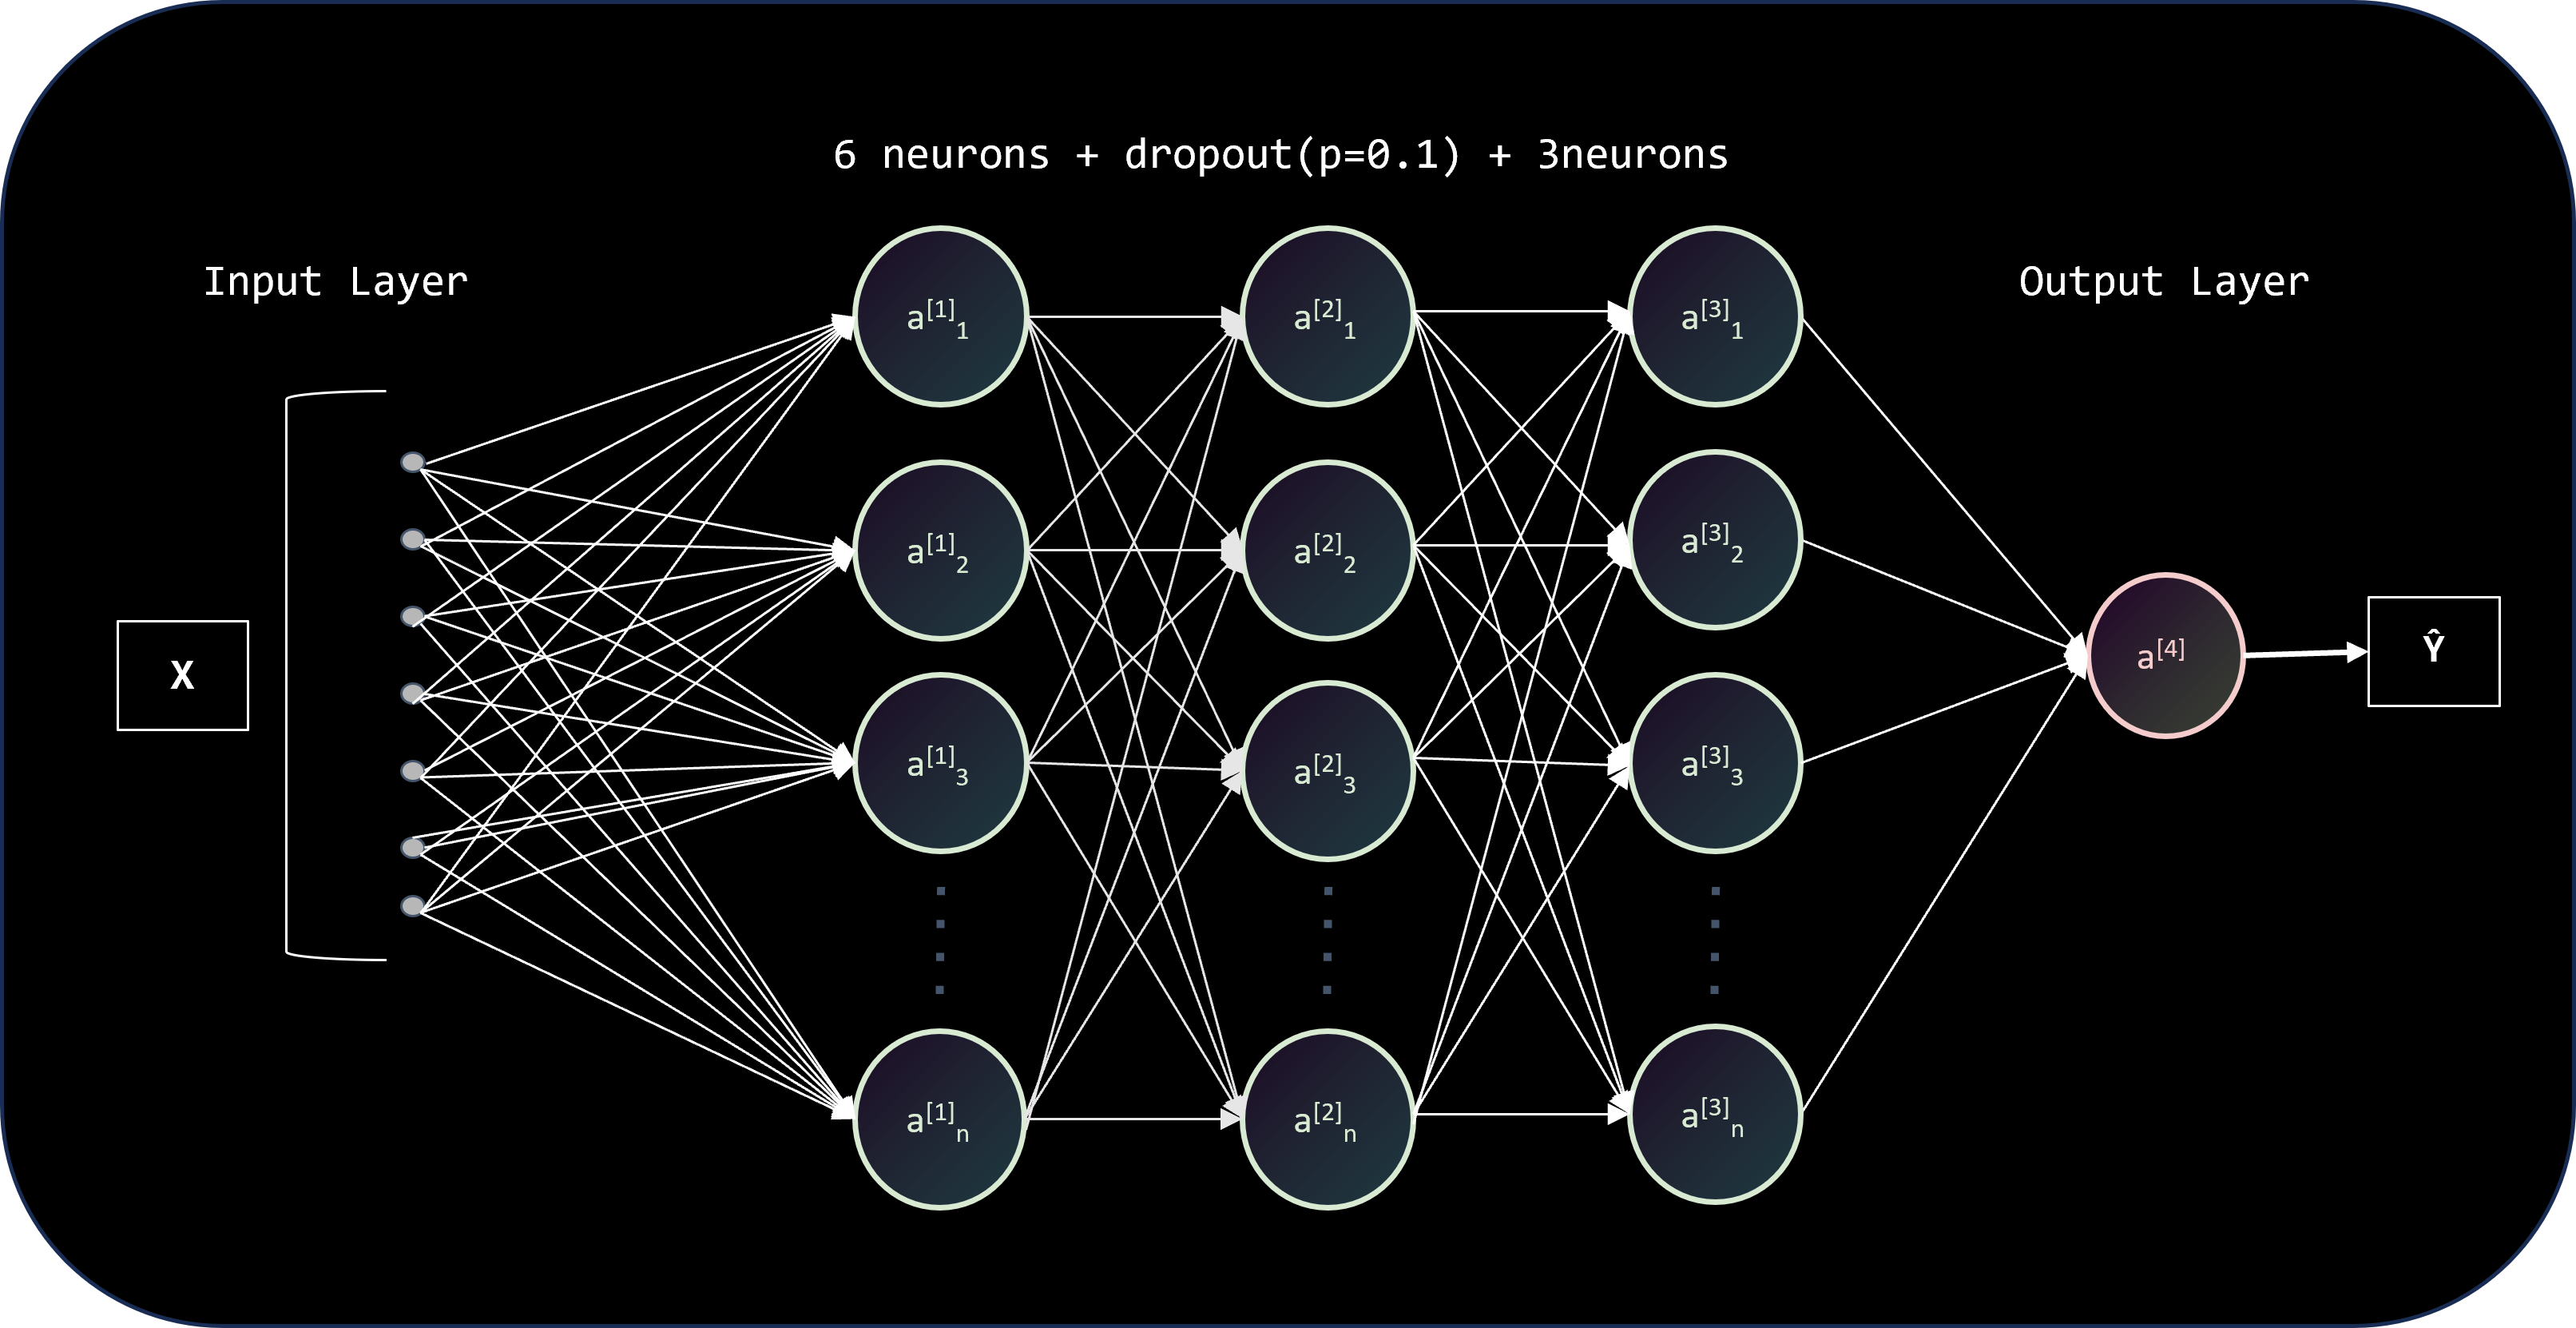
\includegraphics[width=0.5\textwidth]{./figures/nn.png}
	\caption{Backbone MLP of the PW-MLP and PP-MLP}
\end{figure}
\subsection{PW-MLP \& PP-MLP}
\hspace{2em}\textbf{Datasets making.} Our raw datas are selected from \cite{1}. For the PW-MLP set, five elements are chosen as input features, PKPW,BPW, PPPW, FPW, APW respectively. Counterparts for the PP-MLP set are RW, IW, LW. We selected waste quantity and worlds' mitigation on plastics as the label statistics. Datasets are pre-processed with an addition to Gaussian Noises $N(0,0.0001)$, which significantly enlarged samples while maintaining the statistical characteristics.

\textbf{Hyper-params.} We utilize one RTX 4090D 8GB to train the models and employed the regularization techniques to avoid networks' overfittings. The hyper-parameters are set as follows:$\text{batch size}=5, \text{learning rate}=0.0001, \text{Dropout ratio}=0.2, \text{weight decay}=1,\text{epoch}=50$. 

\textbf{MLP-based models.} We choose MLP as our backbone network due to its conciseness and accuracy in prediction missions. Details of PW-MLP and PP-MLP are illustrated in Figure 1, where two hidden layers were deployed, each of which being attached with six and three neurons. Mean Squared Loss was chosen as the loss function while small gradient descent as the optimization algorithm, as is shown in equation \ref{optimization}.
\begin{equation}
	L(\textbf{w},b)=\frac{1}{n}\sum_{i=1}^{\mathbb{B}}\frac{1}{2}(\textbf{w}^T\textbf{x}^{(i)}+b-y^{(i)})^2,\hspace{0.3em}(\textbf{w},b)\leftarrow(\textbf{w},b)-\frac{\eta}{|\mathcal{B}|}\sum_{i\in\mathcal{B}}\partial_{(\textbf{w},b)}l^{(i)}(\textbf{w},b).
	\label{optimization}
\end{equation}

\textbf{Validation of model performance}. We build test datasets similar to the training counterparts and deployed the PP-MLP model to test their generalizability and accuracy. From table \ref{validation} it can be concluded that our model features ideal performance while maintaining strong robustness, meaning that the network is already suitable for prediction mission.

\begin{table}[h]
	\centering
	\begin{tabular}{cccccc}
		\toprule[2pt]
		years & $RW$(mil t) & $IW$(mil t) & $LW$(mil t) & $PPPW_\text{predicted}$(mil t) & $PPPW_\text{real}$(mil t) \\
		\midrule[1pt]
		2010 & 16.87 & 39.28 & 134.1 & 193.85 & 190.25 \\
		2012 & 19.97 & 45.02 & 142.18 & 207.55 & 207.17 \\
		2014& 23.21 & 51.00 & 149.74 & 220.763 & 223.95 \\
		2016 & 27.00 & 57.79 & 159.26 & 236.97 & 244.05 \\
		2018 & 30.93 & 65.31 & 168.32 &  255.96 & 264.56 \\
		2020 & 34.29 & 68.04 & 177.01 & 272.125 & 279.34 \\
		\bottomrule[2pt]
	\end{tabular}
	\caption{Validation of the PP-MLP}
	\label{validation}
\end{table}

\subsection{Plastic Waste Mitigation under PW-MLP and PP-MLP}
\hspace{2em}In our prior notions of $PW$ and $PP$, both variables are defined as: $$PW =\mathcal{F} (PKPW,BPW,PPPW,FPW,APW),PP=\mathcal{L}(RW,IW,LW)$$ which successfully determined the relationship between pivotal parameters and plastic-related features. For instance, from the weights listed in formula \ref{weights}, it can be reached that the $PKPW$ contributes most to the plastic wastes produced annually, aligning with the fact that packaging has long been a crucial component in contemporary industries. 

However, the neural-network-based fitting methodologies itself is insufficient to predict the annual production of plastic wastes, since a majority of the variables bonds tightly with time. Therefore, we mapped the weight matrix into time dimension, enabling the PWM to conduct evaluations over time periods, as is illustrated in formula \ref{map}--\ref{map_2}
\begin{equation}
	\begin{cases}
			PW = \textbf{W}_1^{\top}\cdot\textbf{I}_1,\hspace{0.3em}\text{where}\hspace{0.5em}\textbf{I}_1=\textbf{T}_1(\cdot). \\
		
			PP = \textbf{W}_2^{\top}\cdot\textbf{I}_2,\hspace{0.3em}\text{where}\hspace{0.5em}\textbf{I}_2=\textbf{T}_2(\cdot).
	\end{cases}
	\label{map}
\end{equation}
\begin{figure}[t]
	\centering
	\begin{subfigure}[b]{0.2\textwidth}
		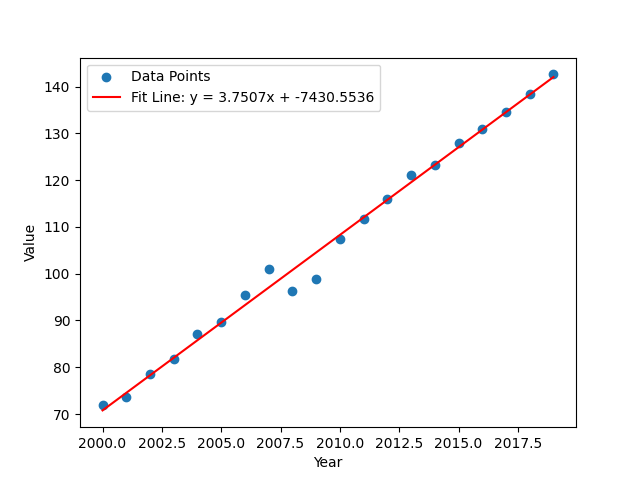
\includegraphics[width=\textwidth]{./figures/alpha_1(t).png}
	\end{subfigure}
	\begin{subfigure}[b]{0.2\textwidth}
		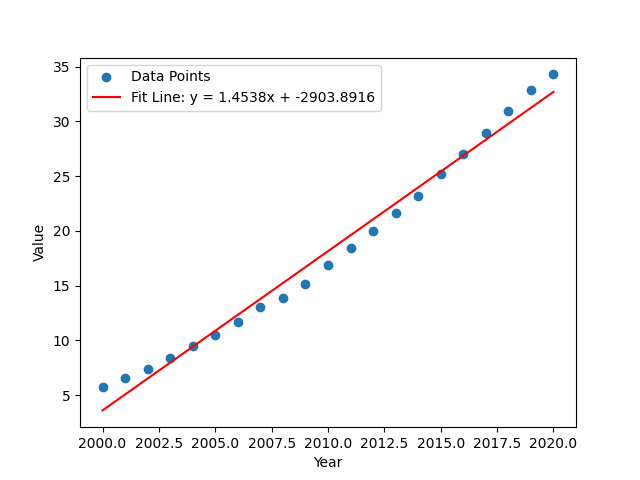
\includegraphics[width=\textwidth]{./figures/alpha_1(t)'.png}
	\end{subfigure}
	\begin{subfigure}[b]{0.2\textwidth}
		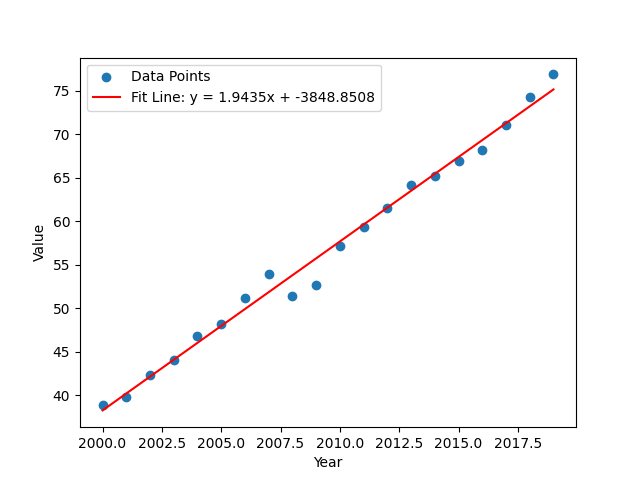
\includegraphics[width=\textwidth]{./figures/beta_2(t).png}
	\end{subfigure}
	\begin{subfigure}[b]{0.2\textwidth}
		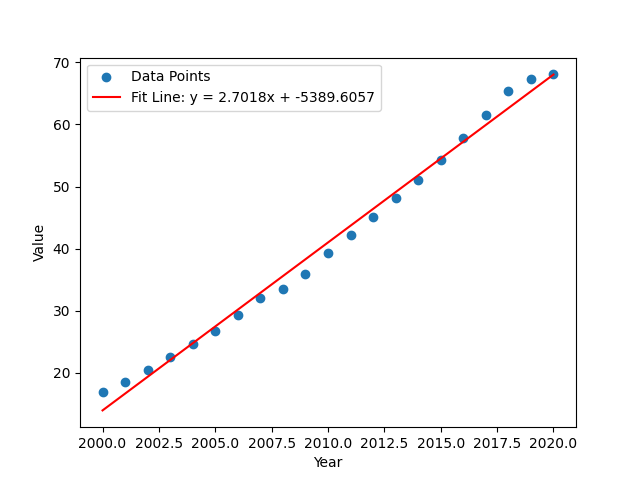
\includegraphics[width=\textwidth]{./figures/beta_2(t)'.png}
	\end{subfigure}
	\begin{subfigure}[b]{0.2\textwidth}
		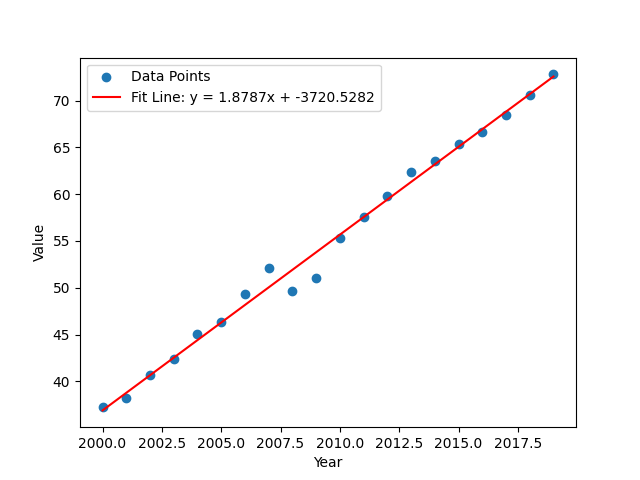
\includegraphics[width=\textwidth]{./figures/gamma_3(t).png}
	\end{subfigure}
	\begin{subfigure}[b]{0.2\textwidth}
		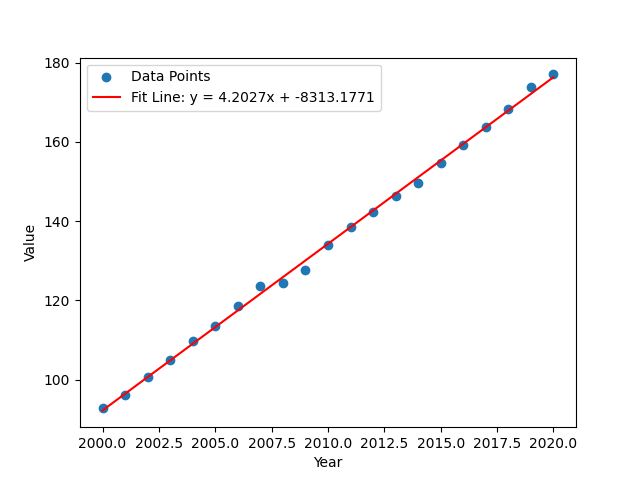
\includegraphics[width=\textwidth]{./figures/gamma_3(t)'.png}
	\end{subfigure}
	\begin{subfigure}[b]{0.2\textwidth}
		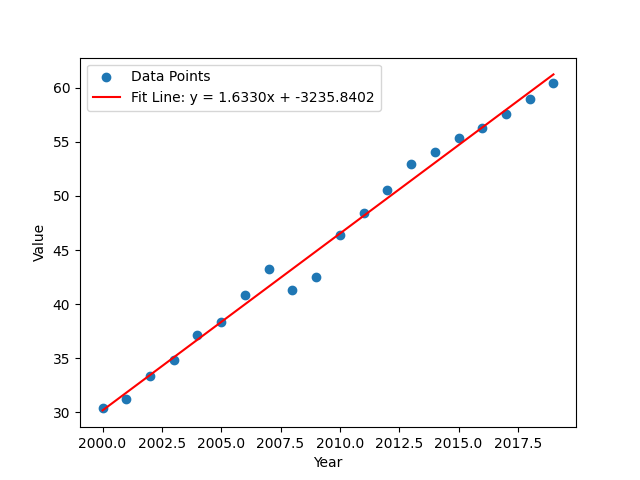
\includegraphics[width=\textwidth]{./figures/theta_4(t).png}
	\end{subfigure}
	\begin{subfigure}[b]{0.2\textwidth}
		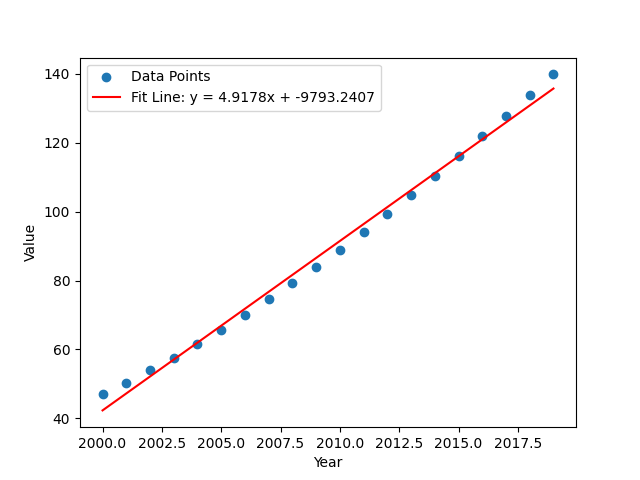
\includegraphics[width=\textwidth]{./figures/epsilon_5(t).png}
	\end{subfigure}
	\caption{Visualization of the linearly fitting process}
	\label{fitting}
\end{figure}
\hspace{2em}Where:
\begin{equation}
		(\textbf{W}_1,\textbf{W}_2)=
		\begin{pmatrix}
			\sigma_1 & \sigma_1' \\
			\sigma_2 & \sigma_2' \\
			\sigma_3 & \sigma_3' \\
			\sigma_4 & 0 \\
			\sigma_5 & 0
		\end{pmatrix}=\begin{pmatrix}
		1.3785 & 0.2300\\ 0.7357 & 0.4620\\ 0.7214 & 1.2811 \\ 0.6039 & 0\\ 0.9428 & 0
		
		\end{pmatrix},\hspace{0.5em}
			(\textbf{I}_1,\textbf{I}_2) = 
		\begin{pmatrix}
				PKPW & RW \\
				BPW & IW \\
				PPPW & LW \\
				FPW & 0 \\
				APW & 0 
		\end{pmatrix}=\begin{pmatrix}
		\alpha_1(t) & \alpha_1'(t) \\
		\beta_2(t) & \beta_2'(t) \\
		\gamma_3(t) & \gamma_3'(t) \\
		\theta_4(t) & 0 \\
		\epsilon_5(t) & 0
		\end{pmatrix}
		\label{weights}
\end{equation}

Then we mapped the Indicator matrix $\textbf{I}$ to time matrix $\textbf{T}(\cdot)$ using \textbf{MATLAB}, producing(figure \ref{fitting}):
\begin{equation}
	(\textbf{I}_1,\textbf{I}_2) = \begin{pmatrix}
		3.75\times t -7430.55 & 1.45\times t-2903.89 \\
		1.94\times t-3848.85 & 2.70\times t-5389.61 \\
		1.88\times t-3720.53 & 4.20\times t-8313.18 \\
		1.62\times t-3235.84 & 0 \\
		4.92\times t-9793.24 & 0 
	\end{pmatrix}
\end{equation}

Hence, we have the original form of PW/PP model, where $PW$ stands for the annual production of plastic wastes and $PP$ stands for humans' capabilities to mitigate the pollution:
\begin{equation}
	\begin{cases}
		PW = 13.5698\times t-26945.79 \\
		PP = 6.9615\times t-13807.91
	\end{cases}
		\label{map_2}
\end{equation}
\hspace{2em}However, 
\ref{map_2} lacks considerations of non-human indicators such as disease outbreaks or technological improvements. We accordingly took the impacts of non-human factors into consideration and introduced the ``non-human coefficient'' to optimize the basic formula, which goes as:
\begin{equation}
	\begin{cases}
		PW = \Theta_1\times13.5698\times t-26945.79+\Delta_1 \\
		PP = \Theta_2\times6.9615\times t-13807.91+\Delta_2 
	\end{cases},\hspace{0.3em}\text{where} \hspace{0.5em}\begin{pmatrix}
	\Theta_1 & \Delta_1 \\
	\Theta_2 & \Delta_2 
	\end{pmatrix}=\begin{pmatrix}
	0.5 & 13240.292 \\
	3 & -41932.37
	\end{pmatrix}
\end{equation}
\hspace{2em}To be specific, $\Theta_1$ and $\Theta_2$ depicts the technological advances in the mitigation of plastic pollution with $\Delta_1$ and $\Delta_2$ being employed make formula $\mathcal{F}(\cdot)$ and $\mathcal{L}(\cdot)$ consistent in $\mathbb{R}$.  The optimized PWM is illustrated in Figure \ref{optimized}.
\begin{figure}[h]
	\centering
	\begin{subfigure}[b]{0.4\textwidth}
		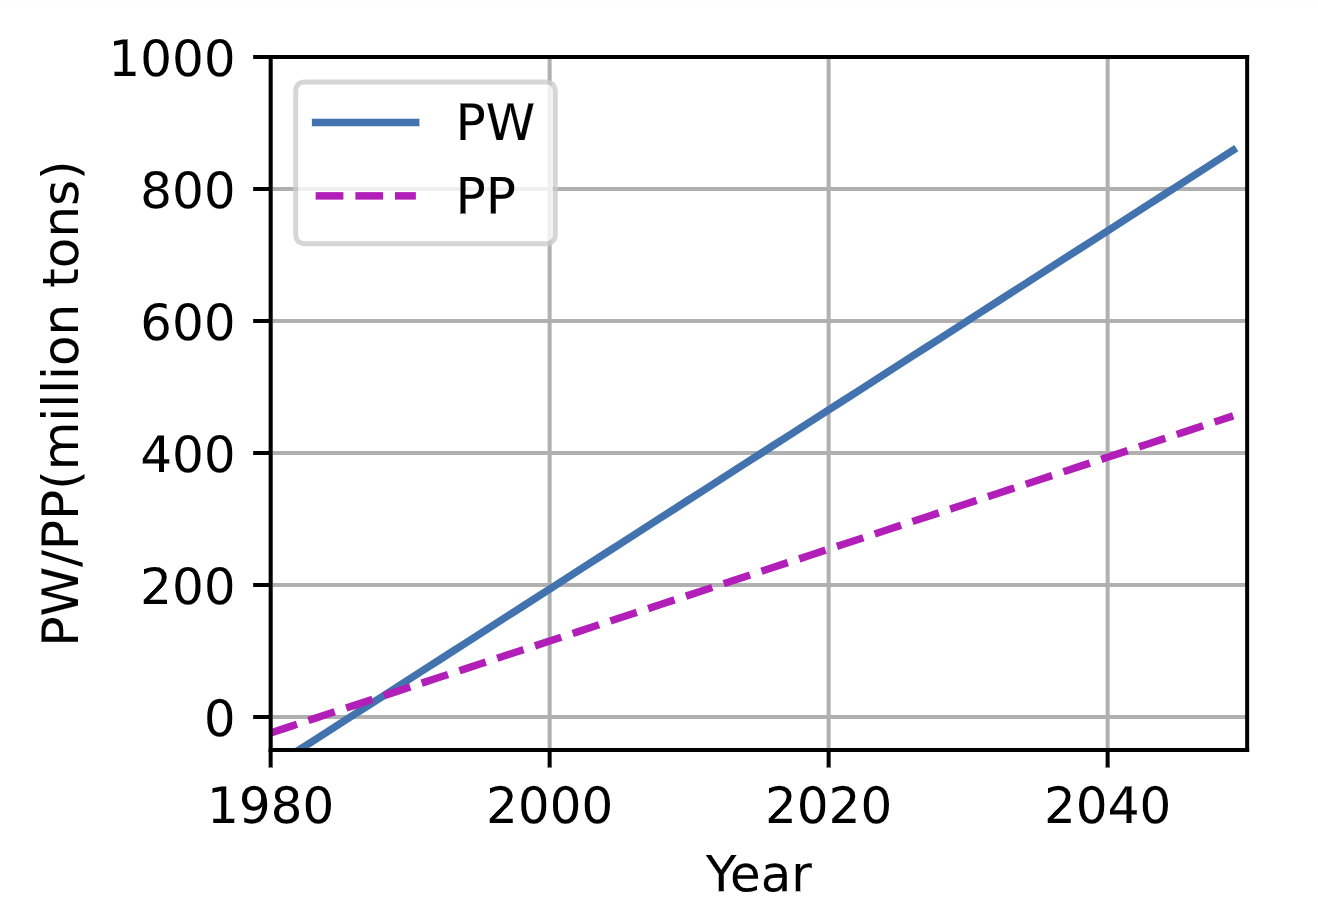
\includegraphics[width=\textwidth]{./figures/original_model.png}
		\caption{primitive form of PW/PP}
	\end{subfigure}
	\begin{subfigure}[b]{0.4\textwidth}
	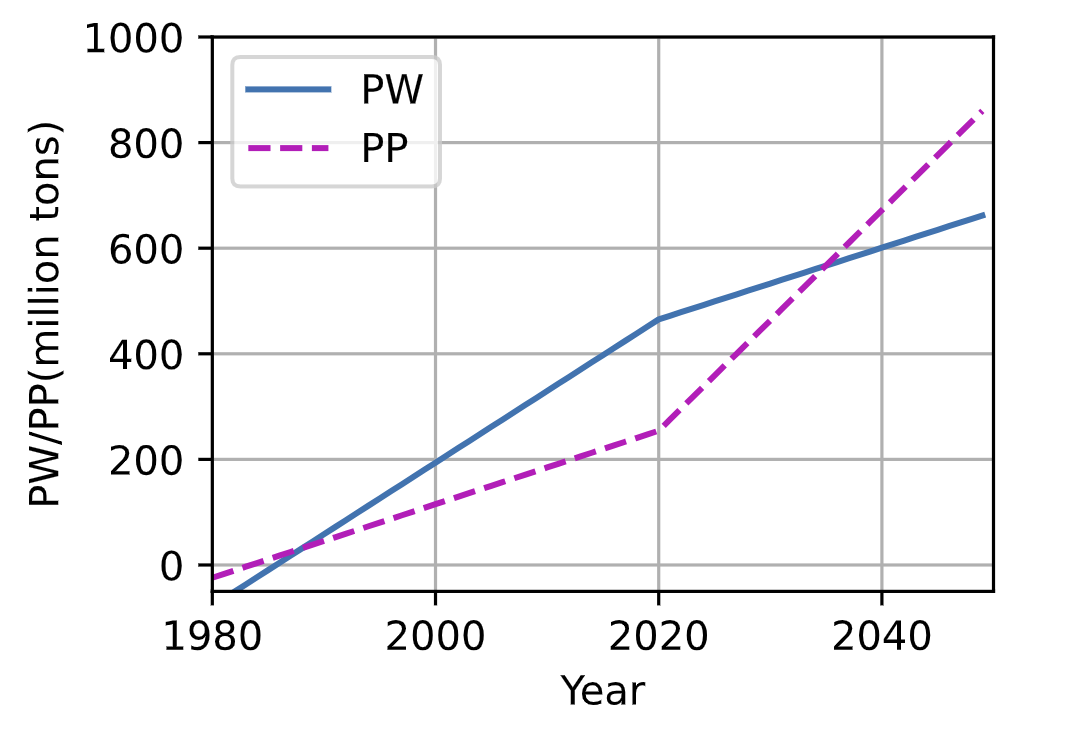
\includegraphics[width=\textwidth]{./figures/optimized_model.png}
	\caption{optimized form of PW/PP}
\end{subfigure}
\caption{Visualization of the PWM.}
\label{optimized}
\end{figure}

According to the PWM model, let $T$ be the year when humans completely reverse the existing trend of plastic waste accumulation, we have:
$$\int_{1983}^{2020}(PW_1-PP_1)dt + \int_{2020}^{2036}(PW_2-PP_2)dt = \int_{2036}^{T}(PW_2-PP_2)dt$$
It can be calculated that $T\approx2052$, which indicates that the existing problem on plastic waste will be fully eliminated in year 2052 as long as humans work in a united fashion and stick closely to the current anti-plastic strategies. Additionally, the intersection of PW and PP means that the plastic waste accumulation could reach a peak  roughly in year 2036, followed by descents in plastic pollution due to advanced technologies. Therefore, it con be concluded that the maximum levels of single-use or disposable plastic product waste that can safely be mitigated without further environmental damage is \textbf{ALL OF THEM}.




%%%%%%%%%%%%%%%%%%%%%%%%%%%%%%
\end{document}
\end
